\Huge\textbf{Capitolo 5: \\Dal DNA alle proteine}

\vspace{1cm}
\small
I geni sono sequenze di DNA che danno origine a proteine, non tutti i geni sono espressi allo stesso modo (solamente quelli codificanti), infatti esistono dei sistemi che ne regolano l'espressione. 
Non tutti i geni sono contemporaneamente espressi, un gene può essere trascritto molteplici volte.\\
L'RNA differisce dal DNA per alcune caratteristiche:
\begin{itemize}
    \item lo zucchero che lo compone è ribosio invece che desossiribosio (è presente un gruppo OH in 2' invece che un H)
    \item viene utilizzata la base uracile al posto della timina (U ha un gruppo H in posizione 5' mentre T ha un CH$_ {3}$), l'appaiamento con A è identico
    \item l'RNA solitamente consiste di un singolo filamento e ha molte forme eterogenee a livello strutturale. 
\end{itemize}

\section{Trascrizione}
    Il processo di trascrizione, ovvero la trascrizione dello stretch di DNA in uno di RNA, avviene grazie ad un melting locale della doppia elica di DNA, l'appaiamento delle basi con la temporanea formazione di un eteroduplex sfruttando l'appaiamento di nucleotidi. 
    Il tutto è mediato dalla RNA polimerasi (RNA-P) che lavora inserendo nucleotidi in 3' in maniera processiva. Solo un filamento di DNA viene utilizzato come filamento stampo.\\
    L'RNA è solitamente composto da poche kb. La formazione dell'eteroduplex trasla con l'avanzamento della RNA-P, non è necessaria la presenza di un primer, non corregge errori (non è grave come per la duplicazione del DNA in quanto si limita alla produzione di un singolo RNA e una singola proteina). 
    Il tasso di errore della RNA-P è di 1 su 10000 (tre ordini di grandezza più frequenti rispetto alla DNA-P).\\
    La sintesi avviene grazie all'idrolisi di ATP (analogamente a quando avviene per la sintesi del DNA).\\
    Solitamente avviene la trascrizione di più molecole di RNA contemporaneamente (ad opera di più RNA-P) da un singolo stretch di DNA. La RNA-P ha una velocità di circa 1.5 kb ogni 50 secondi.\\
    Ci sono molti tipi di RNA differenti, tra i quali \textit{RNA messaggero (mRNA)}, \textit{RNA ribosomiale (rRNA)}, \textit{RNA transfer (tRNA)} e \textit{micro RNA (miRNA)}. Quando si parla di espressione genica si parla della produzione di mRNA.
    
    \subsection{Differenze eucarioti e procarioti}
        Per gli eucarioti la traduzione avviene a livello citoplasmatico mentre la trascrizione a livello del nucleo. Vi è quindi un processo di esportazione dell'mRNA non scontato che passa attraverso i pori della membrana nucleare. Esiste un complesso di esportazione di mRNA maturo al citoplasma per la sua traduzione.\\
        Per i procarioti il ribosoma (per la traduzione) risulta essere nello stesso compartimento del nucleosoma (siccome non vi è una membrana nucleare per la compartimentazione). L'mRNA viene subito in contatto con i ribosomi che traducono la sequenza in proteina.
        
    \subsection{Trascrizione per procarioti}
        \begin{enumerate}
            \item la RNA-P riconosce quale sequenza trascrivere grazie alla presenza della subunità $\sigma$ (\textit{sigma}) che scansiona il duplex e identifica la \textit{sequenza promotore}, composta a 10/35 basi prima dell'effettivo inizio dello stretch da tradurre. 
            \item il complesso di iniziazione di associa stabilmente al DNA.
            \item la subunità $\sigma$ viene rilasciata e inizia la traduzione da parte di RNA-P: questa fase è detta \textit{elongazione}.
            \item RNA-P si dissocia dal filamento nel momento in cui incontra una \textit{sequenza terminatrice}, che viene inclusa nel trascrittto. Si rilascia il mRNA trascitto e la RNA-P si riassocia alla subulità $\sigma$. Questo processo prende il nome di \textit{terminazione}.
        \end{enumerate} 
        Il promotore identifica la direzione 5' a 3' della sequenza. Non viene utilizzato il filamento antiparallelo perchè verrebbero effettivamente prodotte proteine differenti (perchè si andrebbero a leggere codoni complementari).\\
        Geni diversi potrebbero essere trascritti a partire da filamenti diversi.
        \begin{figure}[h]
            \centering
            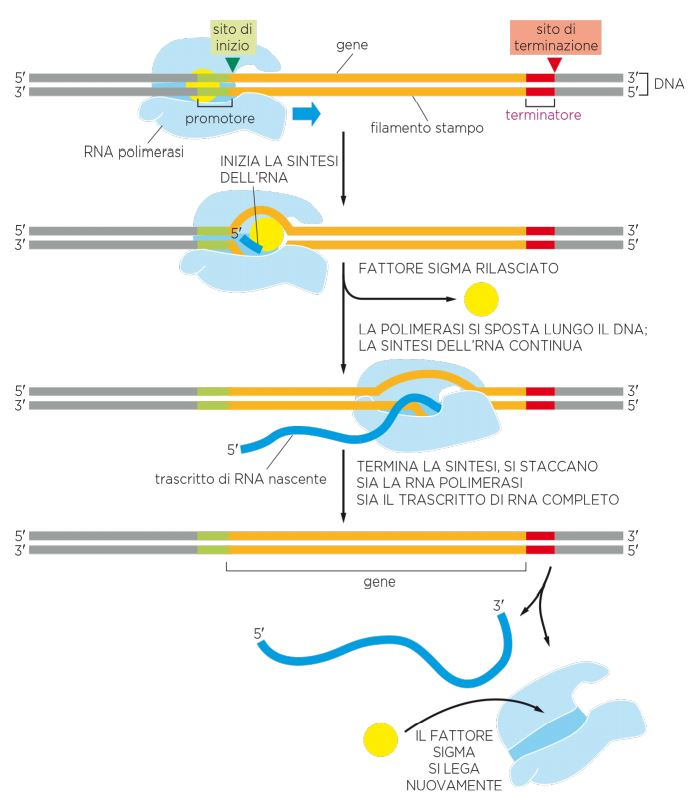
\includegraphics[width=0.4\textwidth]{images/trascrizioneProka.JPG}
            \caption{\small schema delle fasi della trascrizione procariotica}
            \label{fig:mesh1}
        \end{figure}
    
    \subsection{Trascrizione per eucarioti}
        Gli eucarioti hanno RNA-P differenti che assumono compiti specifici:
        \begin{itemize}
            \item RNA-P 1: trascrive la maggioranza del DNA ribosomiale 
            \item \textbf{RNA-P 2}: trascrive geni codificanti proteine 
            \item RNA-P 3: trascrive DNA ribosomiale 5s e tRNA
        \end{itemize}
        Vengono coinvolti altri \textit{transcription factor (TF)}, in particolare (TF II: opera con la RNA-P 2), quali 
        \begin{itemize} 
            \item TF IId è il più simile a $\sigma$ procariotico che utilizza una \textit{TATA binding protein} che si lega alla sequenza nucleotidica della TATA box (a monte della sequenza da trascrivere) che si lega al duplex per reclutare altri componenti specifici
            \item TF IIh: complesso multiproteico (di 9 subunità, compresa una che svolge attività elicasica) che determina la transizione da iniziazione a elongazione tramite attività enzimatica che modifica chimicamente una coda di RNA-P (fosforilazione con CDK7), quindi ne determina la processività.
        \end{itemize}
        Di seguito gli step della trascrizione per le cellule eucariotiche:
        \begin{enumerate}
            \item TF IId si attacca al DNA sulla sequenza specifica della TATA box che viene riconosiuta da TBP (TATA binding protein)
            \item distorsione del sito TATA
            \item formazione del complesso di iniziazione
            \item TF IIh espone il filamento stampo
            \item RNA-P comincia una fase di inizio abortivo (trascrive sequenze che poi vengono scartate fino ad arrivare alla conformazione finale)
            \item avviene la fosforilazione della quinta serina del CTD (ovvero il dominio C-terminale)
            \item RNA-P si stacca da TF IIh e inizia la fase di trascrizione
        \end{enumerate}
        \begin{figure}[h]
            \centering
            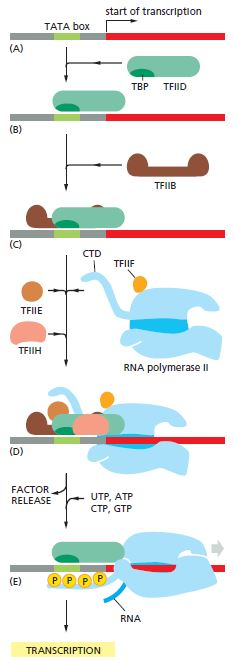
\includegraphics[width=0.3\textwidth]{images/trascrizioneEuka.JPG}
            \caption{\small schema delle fasi della trascrizione eucariotica}
            \label{fig:mesh1}
        \end{figure}
        
        \subsubsection{Maturazione dell'mRNA}
        L'RNA prodotto dalla trascrizione non è ancora pronto per essere utilizzato per la traduzione in proteine. Per la sua maturazione sono necessarie tre ulteriori fasi, ovvero l'apposizione di un capside all'estremità 5', la poliadenilazione all'estremità 3' e il "ritaglio" delle sequenze introniche (slicing). \\
            
            \textbf{Apposizione CAP:}
            Si tratta di una modifica chimica dell'estremità 5'. Viene apposta una metilguanosina da uno specifico enzima tramite un ponte trifosfato 5' - 5'. 
            Questa modifica avviene a livello cotrascrizionale, ovvero avviene durante la trascrizione, approssimativamente dopo circa 25b. Il cap che viene introdotto era precedentemente associato a RNA-P.\\
            
            \textbf{Poliadenilazione:}
            Si tratta di una modifica dell'estremità 3', avviene in contemporanea allo splicing dopo la fine della trascrizione (per ovvi motivi). Viene eliminata una piccola porzione di RNA e viene sostituito con uno stretch di sole adenine (150-250).\\
            Insieme alla presenza del cap in 5' segnala che l'RNA è maturo e pronto per la traduzione.
            
        \vspace{0.5cm}
        Apposizione del CAP e poliadenilazione comportano l'aumento della stabilità dell'RNA (molto instabile e minacciato da RNAasi) e sono necessari per l'esportazione dal nucleo.\\
            
            \begin{figure}[h]
                \centering
                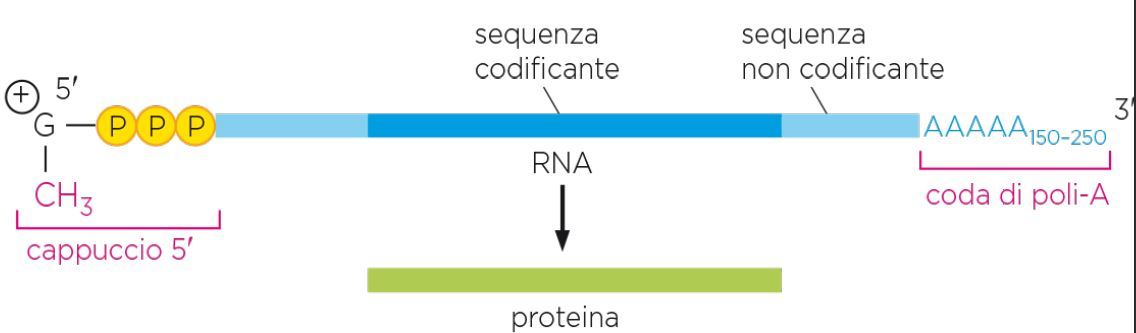
\includegraphics[width=0.5\textwidth]{images/poliAeCap.JPG}
                \caption{\small poliadenilazione e apposizione del CAP}
                \label{fig:mesh1}
            \end{figure}
            
            \textbf{Splicing:}
            Lo splicing è una procedura che avviene solo per gli organismi eucarioti. Infatti il trascritto di RNA contiene delle sequenze non codificanti chiamate \textit{introni}, più lunghe e frequenti di quelle codificanti (\textit{esoni}). 
            Lo splicing si occupa di eliminare queste sequenze lasciando nell'RNA maturo solamente gli esoni.\\
            Lo splicing è una modifica co-trascizionale che avviene tramite una transesterificazione.
            \begin{enumerate}
                \item in corrispondenza di una specifica adenina (solitamente prossima alla fine dell'introne), viene legato il gruppo OH all'estremità 5' del primo nucleotide dell'introne formando una conformazione a \textit{cappio}.
                \item le estremità degli esoni si ricongiungono
                \item viene eliminata la struttura a cappio intronica
            \end{enumerate}
            Un esone comincia sempre per G e finisce per AG, condizione necessaria perchè avvenga lo splicing.
            Un introne contiene sequenze non specifiche ma deve contenere una sequenza al 5' e al 3' specifica e una certa sequenza attorno alla adenina sulla quale avviene la transesterificazione. In particolare viene identificata come \textit{YUR\textbf{A}C}, dove Y sta per una pirimidina e R una purina.\\
            Questo processo è catalizzato da una ribonucleoproteina \textit{snRNP} (\textit{small nuclear ribonucleoprotein}) che si associano singolarmente alle estremità degli introni collaborando alla formazione del cappio e all'intervento di enzimi per lo splicing. \\
            Una volta che il cappio viene eliminato, gli RNA maturi possono formarsi anche cambiando l'ordine delle sequenze esoniche rimaste: questo processo è detto \textit{splicing alternativo} e dà luogo alla formazione di proteine differenti (processo regolato e specifico).
            A livello evolutivo, ci sono domini molto comuni tra proteine diverse e certi altri molto specifici. La modulabilità nella costruzione delle proteine (utilizzo ricorrente di sequenze introniche) aumenta la variabilità delle proteine in modo più efficacie e rapido.
            \begin{figure}[h]
                \centering
                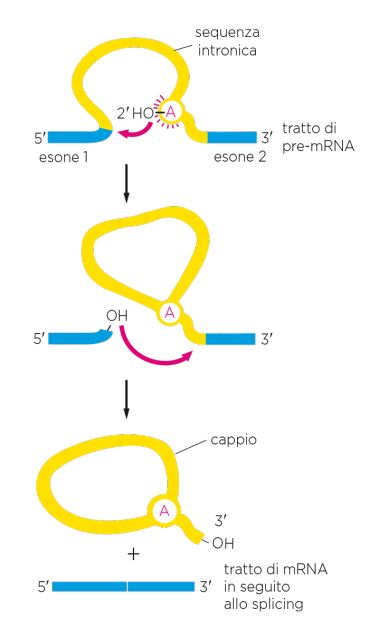
\includegraphics[width=0.4\textwidth]{images/splicing.JPG}
                \caption{\small splicing}
                \label{fig:mesh1}
            \end{figure}
            
        \subsubsection{Esportazione ed emivita}
            Per effettuare lo spostamento dell'mRNA maturo dal nucleo al citoplasma vengono coinvolte numerose proteine che si legano alla testa e alla coda dell'RNA. Ci sono anche complessi di giunzione tra gli esoni. Viene quindi effettuato un legame con il poro nucleare per l'esportazione. \\
            Le stesse proteine promuovono successivamente anche la traduzione. Le componenti che non passano attraverso il poro vengono degradate o riciclate. 
            La sequenza dell'mRNA viene comunque degradata in base alla sua emivita (determinata da sequenze interne codificanti, contribuisce a quest'informazione anche la sequenza in 3' dell'UTR, ovvero \textit{untranslated region}, URT è presente anche al 5'). Dall'emivita dipende il numero di proteine prodotte da quel singolo stretch di mRNA. 

\section{Traduzione}
    Si parla di \textit{traduzione} perchè si passa dal linguaggio nucleotidico a quello AA. Risulta necessario leggere nucleotidi a gruppi di tre in modo da poter riuscire ad identificare univocamente tutti i 20 AA ($4^{3} = 64$ sequenze differenti). Un AA può corrispondere a più triplette (o codoni), tre specifici codoni identificano lo stop alla traduzione.
    Codoni diversi che identificano uno stesso AA sono più variabili all'ultimo nucleotide rispetto agli altri.
    \subsection{Moduli di lettura}
        Ogni proteina comincia con una Metionina, identificata univocamente da AUG (per i mitocondri anche AUA) e finiscono inderogabilmente con una codone di stop (UAA, UAG, UGA). Metionina e stop si possono vedere come elementi di punteggiatura.\\
        Non tutte i nucleotidi dell'mRNA messaggero codificano per AA (per esempio URT citati prima).\\
        Il ribosoma comincia a tradurre la proteina nel momento in cui trova la sequenza AUG per la metionina. Da quel momento legge a gruppi di tre i nucleotidi associando ad ogni tripletta l'AA corretto.
        \subsubsection{Esperimento storico}
            Storicamente, per individuare a quale codone fosse associato quale AA, si creava artificialmente uno stretch di nucleotidi successivo a un mRNA "originale". Per esempio utilizzando uno stretch di U e fornendo questo mRNA sintetico a una cellula, si notava che venivano prodotte fenilalanine. Facendo la stessa cosa con altre sequenze note si riuscirono a dedurre alcuni codoni.\\
            Utilizzando successivamente sequenze di UGUG... alternate si ottiene una sequenza di cisteina e valina, non c'è modo però di sapere se UGU codfichi per l'una o per l'altra.\\
            Successivamente si utilizzarono i tRNA per dedurre la decodifica precisa, da un lato sono coniugate a un AA, dall'altro si associano complementarmente al codone di mRNA. In particolare si utilizzarono delle triplette sintetiche che portarono alla decodifica delle associazioni nucleotidi-AA.
            
    \subsection{tRNA}
        I tRNA sono composti da circa 80 nucleotidi e alla loro estremità in 3' si legano a un AA specifico. Ha una tipica forma a trifoglio e nell'ansa dell'anticodone mostra una sequenza complementare al codone che codifica per l'AA legato al tRNA.\\
        La sua sequenza nucleotidica può contenere basi non canoniche. \\
        I tRNA sono al massimo 61 differenti (64 - 3 codoni di stop), ma il numero minimo è 31. L'uomo possiede solamente 48 tRNA differenti.\\
        La base in posizione 3 è la più variabile (le triplette differenti che codificano per lo stesso AA sono generalmente differenti per il nucleotide in posizione 3). La base azotata \textit{ipoxantina} può comparire in posizione 3 e rappresentare una wildcard per A, C e U. In terza posizione possono esserci anche appaiamenti \textit{wabble} (ad esempio a una C può essere associata una G o una U).
        \begin{figure}[h]
                \centering
                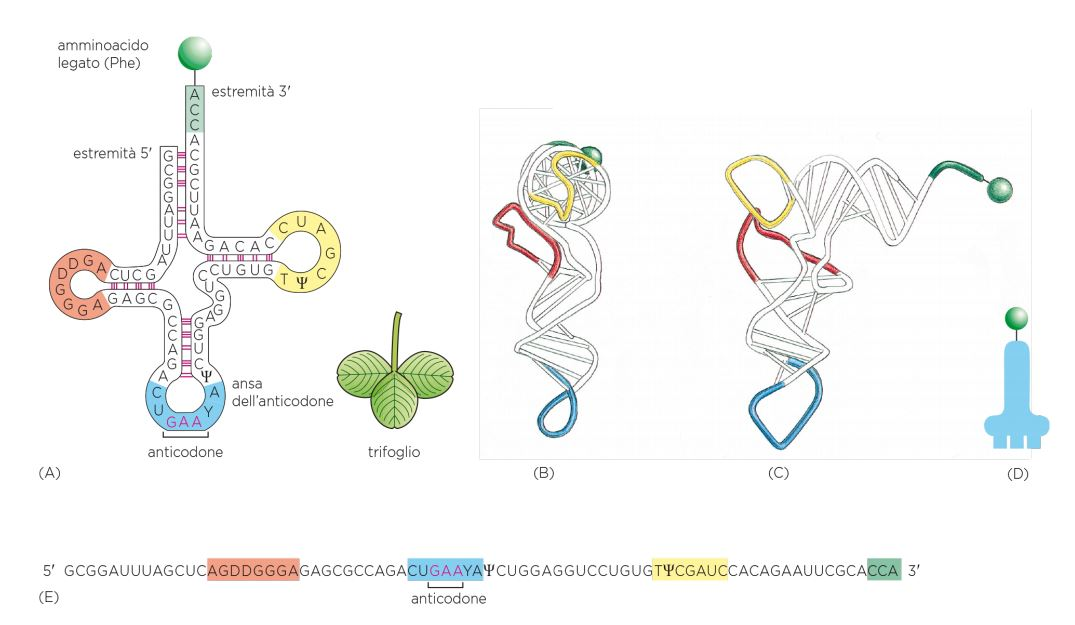
\includegraphics[width=0.5\textwidth]{images/tRNA.JPG}
                \caption{\small tRNA}
                \label{fig:mesh1}
        \end{figure}
    
        \subsubsection{Associazione AA a tRNA}
            Più di un legame ad alta energia viene utilizzato per "caricare" l'AA sul tRNA da una specifica \textit{tRNA sintetasi} per ogni AA. 
            Ogni tRNA sintetasi deve saper riconoscere sequenze di codoni differenti per lo stesso AA e forma un legame estere tra i due. Per il riconoscimento viene utilizzata la sequenza del braccio del trifoglio. 
         
    \subsection{Ribosomi}
        Sono macro-complessi ribonucleoproteici che possono essere libere nel citoplasma o essere associati a RE. Sono formati da 80 proteine differenti e 4 molecole di rRNA. Sono composti di una subunità maggiore (circa 50 peptidi e 3 molecole di rRNA) e una inferiore (circa 30 peptidi e 1 molecola di rRNA). Sulla subunità minore è presente un sito per l'associazione del mRNA.\\
        Tra le due subunità sono presenti tre tasche specifiche (quindi per tre codoni contemporaneamente): E, exit per il rilascio; P, peptidil tRNA e A, amminoacil tRNA. Questi siti coinvolgono sia la subunità maggiore che quella minore. 
        \begin{figure}[h]
                \centering
                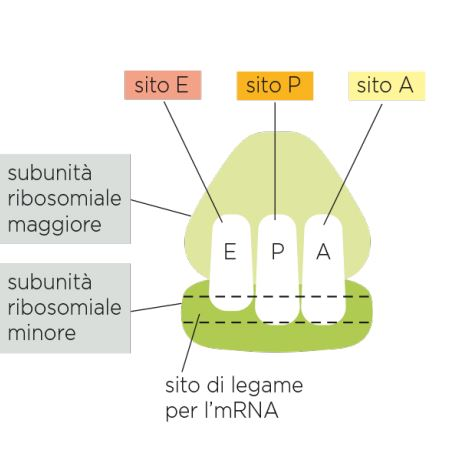
\includegraphics[width=0.35\textwidth]{images/ribosoma.JPG}
                \caption{\small struttura ribosoma}
                \label{fig:mesh1}
        \end{figure}
        Il robozima è la porzione a RNA con funzione catalitica presente del ribosoma che si occupa effettivamente della sintesi proteica, ovvero la \textit{peptidiltransferasi} presente internamente alla subunità maggiore del ribosoma. Strutturalmente è simile a un classico enzima proteico (esiste tasca per favorire la reazione) per orientare i reagenti.
        \subsubsection{Nucleoli}
            Sono domini del nucleo che sintetizzano gli rRNA, tramite RNA-P 1 e 3. C'è una densità di cromatina completamente differente (facilmente osservabili al microscopio) e vengono \textit{clusterizzate} diverse sequenze per il rRNA (cromosoma 1 per rRNA 5s e cromosomi 13, 14, 15, 21 e 22 per rRNA 47s).
    
    \subsection{Processo di traduzione}
        \subsubsection{Inizio per procarioti}
            L'mRNA procariotico maturo non possiede un cap su 5'.
            Esistono sequenze specifiche a cui il ribosoma si associa e comincia la traduzione. Lo stesso mRNA può produrre proteine diverse qualora i ribosomi comincino da AUG differenti (metionine). Gli mRNA batterici che codificano per più geni vengono detti \textit{policistronici}.
        
        \subsubsection{Inizio per eucarioti}
            \begin{enumerate}
                \item La subunità minore si associa ad elementi proteici e a un tRNA iniziatore specifico (che trasporta metionina, riconosce AUG). Esistono due tipi di tRNA per la metionina: uno che viene utilizzato per l'inizio della traduzione e uno per l'inserimento generico di una metionina nella sequenza AA.
                \item Questo complesso si lega all'estremità 5' (riconosciuta dal cap).
                \item Il complesso scorre in direzione 3' fino a trovare il codone AUG per la metionina. Questo evento determina un arresto e quindi il modulo di lettura delle triplette.
                \item I fattori di iniziazione si dissociano e interviene la subunità maggiore del ribosoma per cominciare l'elongazione.
            \end{enumerate}
            Nella maggior parte delle proteine non si riscontra una metionina all'N terminale perchè tramite modifiche post traduzionali vengono spesso rimosse.
            
        \subsubsection{Elongazione}
            \begin{enumerate}
                \item Due tRNA sono ora adiacenti nelle tasche P ed A all'interno del ribosoma. In posizione P, l'AA è legato alla catena peptidica. In posizione A è presente il tRNA che ha portato il nuovo AA da legare al peptide.
                \item Una componente catalitica promuove la formazione del legame peptidico tra l'AA in P e quello in A (reazione catalitica). 
                \item Avviene uno slittamento della subunità maggiore (il sito P diventa E, il sito A diventa P, A rimane vuoto). 
                \item Avviene uno slittamento della subunità minore. Il tRNA che ora era nel sito E viene rilasciato.
                \item Subentra un nuovo tRNA che si associa al codone.
            \end{enumerate}
            Anche la scansione del mRNA avviene dal 5' al 3', per questo abbiamo anche una direzione di sintesi e lettura degli AA (da N a C terminale).\\
            Durante la fase di elongazione avviene anche il folding della proteina. Possono esserci degli chaperon associato al ribosoma. La velocità di sintesi della proteina ha impatto sulla sua conformazione tridimensionale. I tRNA specifici per un codone sono disponibili in quantità differenti, quindi il codone richiesto determina la velocità della sintesi. \\
            Anche gli mRNA possono essere tradotti da poliribosomi, ossia molteplici ribosomi associati allo stesso stretch che traducono la stessa proteina "in fila". Esistono molecole usate come antibiotici che inibiscono la traduzione batterica che non hanno tossicità per i meccanismi umani.
    
        \subsubsection{Terminazione}
            I tRNA antiparalleli ai codoni di stop sono associati a fattori di rilascio.
            \begin{enumerate}
                \item Il sito A contiene una sequenza di stop
                \item Il fattore di rilascio associato al tRNA si lega e cambia conformazione del sito catalitico. Idrolizza il legame tra l'ultimo AA e il suo tRNA rilasciando la proteina neosintetizzata libera. 
                \item Il ribosoma e gli altri fattori si dissociano.
            \end{enumerate}
        
        \begin{figure}[h]
                \centering
                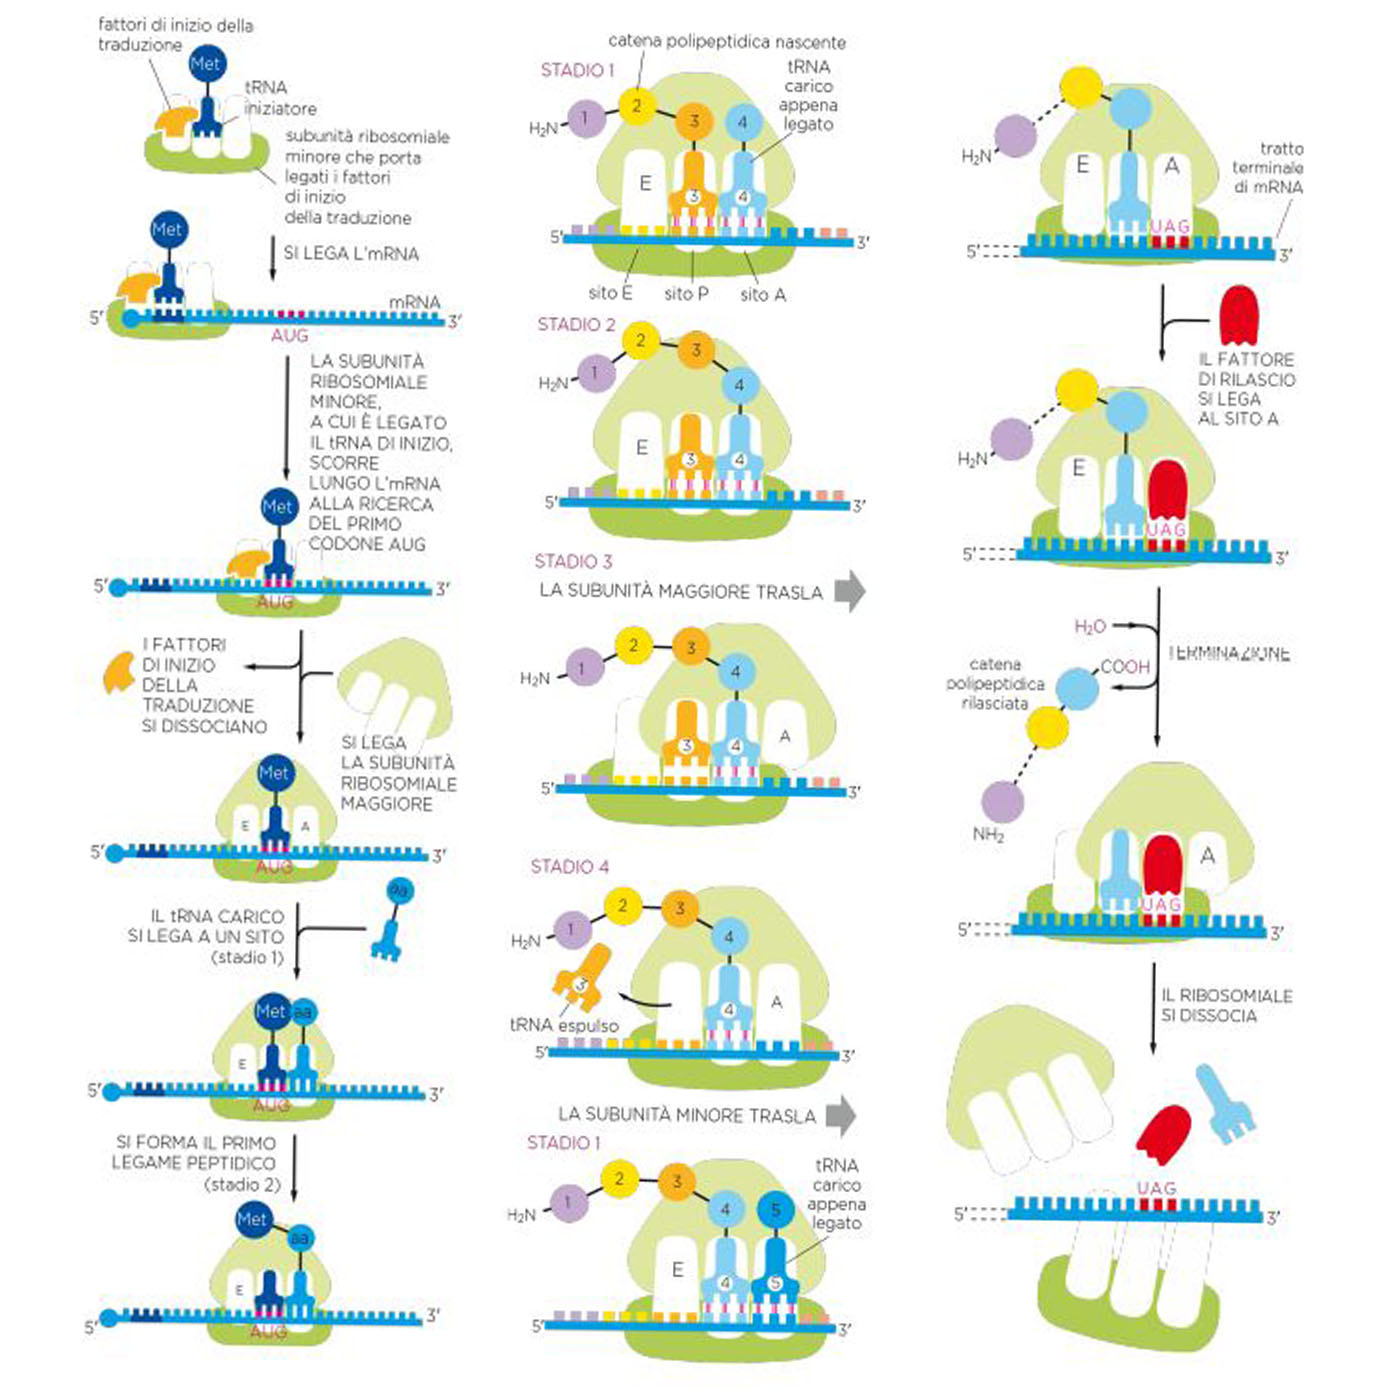
\includegraphics[width=1\textwidth]{images/traduzione.jpg}
                \caption{\small fasi della traduzione, rispettivamente iniziazione, elongazione e terminazione per gli eucarioti}
                \label{fig:mesh1}
        \end{figure}
        
        \subsubsection{Post traduzione e morte}
            Le proteine possono subire delle modifiche post-traduzionali, ne si può modificare l'emivita e di conseguenza la sua concentrazione. \\
            Un polipeptide che finisce il suo ciclo di vita viene "spezzettato" nel proteasoma, un core catalitico che svolge il polipeptide (consumando ATP) e rilascia AA singoli o bipeptidi nel citoplasma.\\
            L'ubiquitina è un marker per le proteine che devono essere degradate, l'aggiunta molteplici catene di questa proteina (composta di 76 AA) è anche essa una modifica post-traduzionale chiamata \textit{poliubiquitinazione} e viene effettuata sempre su una lisina.\\
            Il proteasoma riconosce le sequenze di ubiquitina e degrada la proteina.\\ 

\pagebreak